МРНТИ 20.20.20

\sectionwithauthors{Т.Ж. Мазаков, Ш.А. Джомартова, А.Т. Мазакова, Т.С. Шорманов, М.С. Алиаскар}{ГИБРИДНАЯ МОДЕЛЬ ПРОГНОЗИРОВАНИЯ ПРОЦЕССА СЕЛЕВОГО ПРОРЫВА}

\begin{center}
{\bfseries \textsuperscript{1,2}Т.Ж. Мазаков, \textsuperscript{1}Ш.А.
Джомартова, \textsuperscript{1}А.Т. Мазакова, \textsuperscript{1}Т.С.
Шорманов, \textsuperscript{1,2}М.С. Алиаскар}

\textsuperscript{1}Казахский национальный университет имени аль-Фараби,
Алматы, Казахстан,

\textsuperscript{2}Международный инженерно-технологический университет,
Алматы, Казахстан,

e-mail: tmazakov@mail.ru
\end{center}

Целью данной работы является разработка гибридной модели прогнозирования
последствий селевого прорыва гидротехнических сооружений, таких как
дамбы и плотины. Представленная работа посвящена автоматизации процессов
моделирования и анализа разрушения гидротехнических сооружений,
основываясь на современных методах гидродинамики и теплофизики.
Актуальность данной работы обусловлена увеличением частоты и масштаба
катастрофических наводнений, вызванных разрушением гидротехнических
сооружений, что требует эффективных методов прогнозирования и
предотвращения подобных событий. Предложенные в работе методы и модели
имеют значительное практическое значение для оценки рисков, планирования
эвакуационных мероприятий и минимизации ущерба от чрезвычайных ситуаций,
связанных с прорывами плотин и дамб.

{\bfseries Ключевые слова}: гидротехнические сооружения, прорыв плотины,
селевой поток, численное моделирование, интервальная математика,
прогнозирование.

\begin{center}
{\large\bfseries СЕЛДІҢ СЕРПІЛІС ПРОЦЕСІН БОЛЖАУҒА АРНАЛҒАН ГИБРИДТІ МОДЕЛЬ}

{\bfseries \textsuperscript{1,2}Т.Ж. Мазаков, \textsuperscript{1}Ш.А.
Джомартова, \textsuperscript{1}А.Т. Мазакова, \textsuperscript{1}Т.С.
Шорманов,}

{\bfseries \textsuperscript{1,2}М.С. Әлиасқар}

\textsuperscript{1}Әл-Фараби атындағы Қазақ ұлттық университеті, Алматы,
Қазақстан,

\textsuperscript{2}Халықаралық инженерлік-технологиялық университеті,
Алматы, Қазақстан,

e-mail: tmazakov@mail.ru
\end{center}

Бұл жұмыстың мақсаты дамбы мен бөгеттер сияқты гидротехникалық
құрылыстардың сел серпілісінің салдарын болжаудың гибридті моделін жасау
болып табылады. Ұсынылған жұмыс гидродинамика мен термофизиканың
заманауи әдістеріне негізделген гидротехникалық құрылыстардың бұзылуын
модельдеу және талдау процестерін автоматтандыруға арналған. Бұл
жұмыстың өзектілігі гидротехникалық құрылыстардың бұзылуынан туындаған
апатты су тасқындарының жиілігі мен ауқымының артуына байланысты, бұл
мұндай оқиғаларды болжау мен алдын алудың тиімді әдістерін қажет етеді.
Жұмыста ұсынылған әдістер мен үлгілердің қауіп-қатерді бағалау,
эвакуациялау шараларын жоспарлау және бөгет пен бөгеттің бұзылуымен
байланысты төтенше жағдайлардан залалдарды азайту үшін маңызды
практикалық маңызы бар.

{\bfseries Түйін сөздер:} гидротехникалық құрылыстар, бөгеттердің жарылуы,
сел, сандық модельдеу, интервалдық математика, болжау.

\begin{center}
{\large\bfseries Hybrid model for predicting the mudflow breakthrough process}

{\bfseries \textsuperscript{1,2}T.Zh. Mazakov, \textsuperscript{1}Sh.A.
Jomartova, \textsuperscript{1}A.T. Mazakova, \textsuperscript{1}T.S.
Shormanov,}

{\bfseries \textsuperscript{1,2}M.S. Aliaskar}

\textsuperscript{1}Al-Farabi Kazakh National University, Almaty,
Kazakhstan,

\textsuperscript{2}International Engineering Technological University,

е-mail: tmazakov@mail.ru
\end{center}

The purpose of this work is to develop a hybrid model for predicting the
consequences of a mudflow breakthrough of hydraulic structures, such as
dams and dams. The presented work is devoted to the automation of the
processes of modeling and analysis of the destruction of hydraulic
structures, based on modern methods of hydrodynamics and thermophysics.
The relevance of this work is due to the increasing frequency and scale
of catastrophic floods caused by the destruction of hydraulic
structures, which requires effective methods for predicting and
preventing such events. The methods and models proposed in the work are
of significant practical importance for risk assessment, planning
evacuation measures and minimizing damage from emergencies associated
with dam and dam breaks.

{\bfseries Key words:} hydraulic structures, dam break, mudflow, numerical
modeling, interval mathematics, forecasting.

\begin{multicols}{2}
{\bfseries Введение.} При прорыве дамбы (плотины) в зависимости от скорости
объема водоема, высоты плотины, перепада рельефа местности выделены
четыре зоны катастрофического затопления (рисунок 1). Первая зона
(бурного течения) начинается от основания плотины и простирается на 6-15
километров. Высота волны в этой зоне может достигать нескольких метров.
Скорость течения потока воды находится в пределах от 20 км/ч и выше.
Время прохождения волны -- 30 минут. Протяженность второй зоны (быстрого
течения) может быть в пределах 15-25 км от основания плотины. Время
прохождения волны -- 60 минут. Скорость течения потока воды находится в
пределах 15-20 км/ч. Протяженность третьей зоны (среднего течения) может
быть в пределах 25-35 км от основания плотины. Время прохождения волны
-- 2-3 часа. Скорость течения потока воды находится в пределах 10-15
км/ч. Протяженность четвертой (слабого течения) может быть в пределах
36-70 км от основания плотины и зависит от рельефа местности. Скорость
течения потока воды находится в пределах 6-10 км/ч {[}1{]}.
\end{multicols}

\begin{figure}[H]
	\centering
	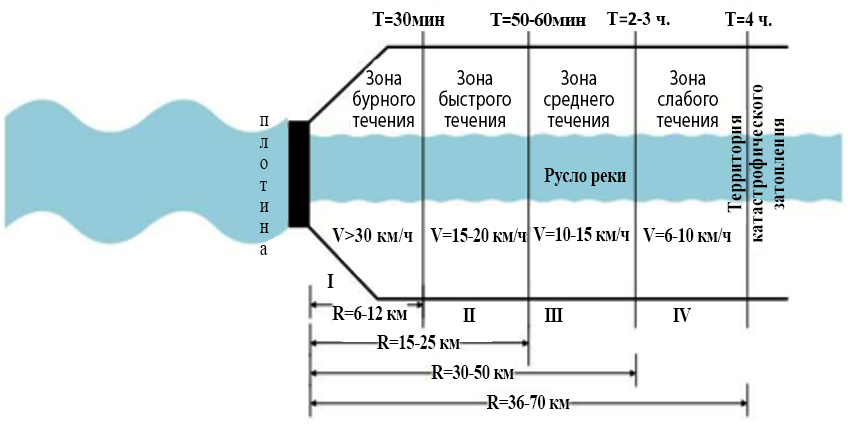
\includegraphics[width=0.8\textwidth]{assets/61}
	\caption*{Рис. 1 -- Зоны катастрофического затопления}
\end{figure}

{\bfseries Материалы и методы.} \emph{Одномерные математические модели.}

\emph{Модель A.M. Прудовского}

Расчет проводится для каждого расчетного створа и основан на значениях
ряда фиксированных таблиц {[}2{]}. Определяются время прихода гребня
(\(t_{гр}\)) и фронта (\(t_{фр}\)) волны, высота (h) и скорость (V)
волны прорыва:

\begin{equation}
h = \frac{A_{h}}{\sqrt{B_{h} + L}},\ \text{м}\qquad V = \frac{A_{v}}{\sqrt{B_{v} + L}},\ \text{м/с}
\end{equation}

где L -- удаленность створа объекта от ГТС, км;

I -- гидравлический уклон, определяемый по карте;

\(h_{M}\) -- высота местности, м;

\(h_{\delta}\) -- глубина реки в нижнем бьефе, м;

\(H_{0}\) -- высоты уровня воды в верхнем бьефе плотины.

Определяется продолжительность времени затопления территории по формуле:

\begin{equation}
\tau = \beta \cdot \left( t_{\text гp} - t_{\text фp} \right) \cdot \left( 1 - \frac{h_{\text м}}{h} \right)\text{, час}
\end{equation}

где β -- коэффициент, зависящий от высоты плотины, гидравлического
уклона и расстояния до объекта {[}3{]}.

\emph{Модель Исмагилова Х.А.}

\begin{equation*}
B = \left( \frac{1 + S}{f_{\text кp}} \right)^{1,33}\frac{Q_{p}^{0,6}}{d^{0,25}(gi)^{0,25}},\qquad
H = 0,62f_{\text кp}(1 + S)\frac{Q_{p}^{0,25}d^{0,375}}{(gi)^{0,125}}
\end{equation*}

\begin{equation}
\frac{H}{B} = \frac{0,62f_{\text кp}^{2,23}}{{(1 + S)}^{0,33}}\frac{d^{0,625}(gi)^{0,125}}{Q_{p}^{0,25}}
\end{equation}

где $B$ -- ширина русла, м;

$H$ -- глубина потока, м;

\(Q_{p}\) -- расчетный селевой расход, \(м^{3}/с\);

$S$ -- объемная мутность;

\(f_{кр}\) -- коэффициент крепости грунта на деформацию;

$i$ -- уклон русла;

$d$ -- средний диаметр донных отложений {[}4{]}.

\emph{Модель Секисовой И.А.}

\begin{equation}
h_{\max} = 2,51\frac{H_{0}^{0,98}n_{0}^{0,02}Q_{0}^{0,05}}{W_{\text{вод}}^{0,05}L^{0,13}}
\end{equation}

\begin{multicols}{2}
В (4) объем водохранилища до начала аварии (\(W_{\text{вод}}\)), глубина
водохранилища у плотины до начала аварии (\(H_{0}\)), шероховатость
русла верхнего бьефа (\(n_{0}\)), величина раскрытия прорана
(\(B_{\text{пр}}\)), расход воды в нижнем бьефе гидроузла до начала аварии
(\(Q_{0}\)), расстояние от створа плотины до створа наблюдения (L).

Границы применимости формулы (5): \(W_{\text{вод}}\) -- от 50 до 5000 тыс.
м\textsuperscript{3}; \(H_{0}\) -- от 2 до 20 м; \(Q_{0}\) -- от 1 до
100 м\textsuperscript{3}/с; длина водохранилища -- от 0,8 до 2 км; $L$ от
0,5 до 50 км; \(n_{0}\) от 0,02 до 0,2 {[}5{]}.
\end{multicols}

\emph{Модель Волкова}

\begin{equation}
h_{\max} = 0,34H_{0}\left( \frac{L}{H_{0}} \right)^{- 0,13}
\end{equation}

\emph{Недостатки вышеприведенных методик.}

\begin{multicols}{2}
В (4) отсутствует параметр -- величина раскрытия прорана (\(B_{\text{пр}}\)),
объем водохранилища до начала аварии (\(W_{\text{вод}}\)), размещен в
знаменателе, что приводит к противоречию основам гидрологии -- «больший
объем заполненности водоема приводит к уменьшению волны прорыва».

В (5) не используются такие важные параметры ГТС как объем водохранилища
до начала аварии (\(W_{\text{вод}}\)), величина раскрытия прорана (\(B_{\text{пр}}\)).
\end{multicols}

Наша формула:

\begin{equation}
h_{\max} = 1,34*H_{0}^{0,55}B_{\text{пр}}^{0,32}W_{0}^{0,04}L^{- 1,4}\cos(\theta )
\end{equation}

\begin{multicols}{2}
В формуле (6) объем водохранилища (\(W_{\text{вод}}\)) измеряется в миллионах
м\textsuperscript{3}; глубина воды в верхнем бьефе у плотины (\(H_{0}\))
-- в м; величина раскрытия прорана (\(B_{\text{пр}}\)) -- в м; расстояние от
створа плотины до створа наблюдения (L) -- в км, \(\theta\) - в
градусах.

\emph{Границы применимости формулы (6)} (связанные с методикой его
обоснования): объем водохранилища (\(W_{\text{вод}}\)) -- от 3
млн.м\textsuperscript{3} и выше; высота плотины (\(H_{0}\)) -- от 3 м и
выше; расстояние от створа плотины до створа наблюдения (L) -- от 3 м и
выше. Указанные ограничения не препятствуют практическим интересам
{[}6-7{]}.

{\bfseries Результаты и обсуждение.} \emph{Трехмерные математические
модели.}

Все существующие программные пакеты можно разделить на одно-, двух- и
трехмерные. Одномерное или двумерное численное моделирование значительно
упрощает исследуемые модели и не дает полного понимания процессов,
связанных с разрушением волн и распространением паводковых волн, как
будет показано ниже. Поэтому наиболее точным применением трехмерного
численного моделирования является расчет затопления и разрушения волн.

Далее будем исследовать трехмерные задачи. С этой целью введем
xyz-систему координат, ориентировав ее следующим образом: z-ось
направлена в верх и характеризует высоту волны прорыв, y-ось описывает
ширину зоны прорыва и обычно ограничена рельефом местности (ширина
ущелья), x-ось характеризует направление прорыва и отсчитывается,
начиная от стены плотины. На рисунке 2 показано ее применение на примере
реки Есик (Республика Казахстан).
\end{multicols}

\begin{figure}[H]
	\centering
	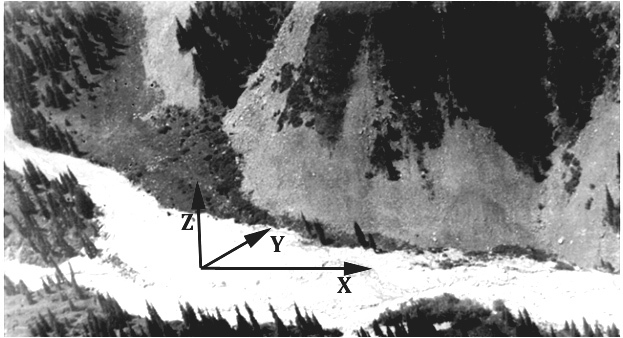
\includegraphics[width=0.8\textwidth]{assets/62}
	\caption*{Рис. 2 - Зона реки Есик}
\end{figure}

\begin{multicols}{2}
В большинстве случаев базовой системой гидродинамического моделирования
является трехмерная система эволюционирующих уравнений Навье-Стокса. В
математике уравнения Навье-Стокса представляют собой систему нелинейных
дифференциальных уравнений для абстрактных векторных полей произвольной
величины. Это уравнение является формулировкой второго закона Ньютона
{[}8{]}.

Уравнения движения:
\end{multicols}

\begin{equation}
\frac{\partial u}{\partial t} + \frac{\partial(u^{2})}{\partial x} + \frac{\partial(uv)}{\partial y} + \frac{\partial(uw)}{\partial z} = \frac{\partial P}{\partial x} + \frac{1}{\Re}\left( \frac{\partial^{2}u}{\partial x^{2}} + \frac{\partial^{2}u}{\partial y^{2}} + \frac{\partial^{2}u}{\partial z^{2}} \right),
\end{equation}

\begin{equation}
\frac{\partial v}{\partial t} + \frac{\partial(uv)}{\partial x} + \frac{\partial(v^{2})}{\partial y} + \frac{\partial(vw)}{\partial z} = \frac{\partial P}{\partial y} + \frac{1}{\Re}\left( \frac{\partial^{2}v}{\partial x^{2}} + \frac{\partial^{2}v}{\partial y^{2}} + \frac{\partial^{2}v}{\partial z^{2}} \right),
\end{equation}

\begin{equation}
\frac{\partial w}{\partial t} + \frac{\partial(uw)}{\partial x} + \frac{\partial(vw)}{\partial y} + \frac{\partial(w^{2})}{\partial z} = \frac{\partial P}{\partial z} + \frac{1}{\Re}\left( \frac{\partial^{2}w}{\partial x^{2}} + \frac{\partial^{2}w}{\partial y^{2}} + \frac{\partial^{2}w}{\partial z^{2}} \right),
\end{equation}

где \(u = u(x,y,z,t),\ v = v(x,y,z,t),\ w = w(x,y,z,t)\) -- проекции
неизвестной функции скорости \(V\) на оси \(x,\ y,\ z\) d декартовой
прямоугольной трехмерной системе координат: \(P = P(x,y,z,t)\) --
неизвестная функция давления: \(Re\) -- число Рейнольдса.

Уравнение неразрывности:

\begin{equation}
\frac{\partial u}{\partial x} + \frac{\partial v}{\partial y} + \frac{\partial w}{\partial z} = 0.,
\end{equation}

\begin{multicols}{2}
\(u\) -- \(X\)-компонента вектора скорости \(\overrightarrow{v}\);

\(v\) -- \(Y\)-компонента вектора скорости \(\overrightarrow{v}\);

\(f_{x}\) -- \(X\)-компонента вектора внешних сил
\(\overrightarrow{f}\);

\(f_{y}\) -- \(Y\)-компонента вектора внешних сил
\(\overrightarrow{f}\);

\(\Re\) -- число Рейнольдса, безразмерная величина {[}9{]}.

Применение модели Навье-Стокса для исследовании задачи прорыва плотины
носит больше всего теоретический интерес. Для численного нахождения
решения задачи (7)-(9) существуют множество алгоритмов и программных
продуктов. Однако при их применении требуются достаточные объемы
оперативной памяти и достаточно долгое ожидание окончательного решения.
К модели (7)-(9) тяжело привязать реальный рельеф местности. В процессе
вытекания селевая жидкость представляет собой грязную смесь, состоящую
из воды, камней и других веществ, захватываемых в процессе протекания
сели.

Для практики важны чтобы применяемая математическая модель отвечала
следующим требованиям: 1) могла быть реализована на микропроцессорной
технике, 2) находила решение за приемлемое время, 3) в режиме реального
времени могла бы уточняться.

По большому счету с точки зрения практики не важно с какой скоростью
движется точка с xyz-координатами в каждый момент времени t. Больший
интерес представляет высота волны на плоскости в точке с xy-координатами
в определенный момент времени t {[}10{]}.

Наша модель является гибридной и состоит из двух частей:

первая описывает максимально возможное значение высоты волны прорыва в
точке отстоящей на расстоянии L от плотины и описывается следующим
уравнением
\end{multicols}

\begin{equation}
h_{\max} = 1,34*H_{0}^{0,55}B_{пр}^{0,32}W_{0}^{0,04}L^{- 1,4}\cos(\theta)
\end{equation}

вторая описывает динамику прорывной волны на плоскости и представляет
собой двумерное уравнение Навье-Стока

\begin{equation}
\frac{\partial u}{\partial t} + \frac{\partial(u^{2})}{\partial x} + \frac{\partial(uv)}{\partial y} = \frac{\partial P}{\partial x} + \frac{1}{\Re}\left( \frac{\partial^{2}u}{\partial x^{2}} + \frac{\partial^{2}u}{\partial y^{2}} \right),
\end{equation}

\begin{equation}
\frac{\partial v}{\partial t} + \frac{\partial(uv)}{\partial x} + \frac{\partial(v^{2})}{\partial y} = \frac{\partial P}{\partial y} + \frac{1}{\Re}\left( \frac{\partial^{2}v}{\partial x^{2}} + \frac{\partial^{2}v}{\partial y^{2}} \right),
\end{equation}

\begin{equation}
\frac{\partial u}{\partial x} + \frac{\partial v}{\partial y} = 0.
\end{equation}

\begin{multicols}{2}
Уравнения (12)-(14) позволяют нам оценить нахождение фронта прорыва
(первой волны).

Общий алгоритм можно представить следующим образом:

Шаг 1. Производим установку начальных и краевых условий. Пусть tn=0;

Шаг 2. tk=tn+dt; Для момента времени tk решается плоскостная задача
Навье-Стокса (12)-(14).

Шаг 3. Определяется граница нахождения первой волны прорыва.

Шаг 4. Для всех плоскостных точек волны прорыва с координатами xy
вычисляется расстояние до плотины. Затем по формуле (10) вычисляется
максимально возможное значение высоты волны.

Шаг 5. tn= tk. Определяется нужно ли продолжать вычисления для нового
времени. Если «ДА», то переход к шагу 2.

Предложенный алгоритм программно реализован и в настоящее время проходит
экспериментальные вычисления.

Работа выполнена за счет средств НИИ математики и механики при КазНУ
имени аль-Фараби и грантового финансирования научных исследований на
2023--2025 годы по проекту AP19678157.

{\bfseries Выводы.} В данной работе была разработана гибридная модель
прогнозирования процесса селевого прорыва, сочетающая аналитические и
численные методы решения задач гидродинамики и теплофизики.
Разработанный алгоритм позволяет более точно моделировать процессы
разрушения плотин и распространения селевых волн, что имеет важное
практическое значение для предотвращения катастрофических затоплений.

Результаты численных расчетов показывают, что предложенная модель может
эффективно применяться для прогнозирования параметров селевых потоков и
определения зон затопления. Программа, реализующая данный алгоритм,
демонстрирует высокую точность и надежность расчетов, что подтверждается
сравнением с существующими моделями и экспериментальными данными.

Перспективы дальнейших исследований включают применение интервальной
математики для более точного анализа уравнений теплопроводности, а также
интеграцию разработанной модели с современными системами мониторинга и
предупреждения о чрезвычайных ситуациях. Это позволит повысить
эффективность мер по защите населения и инфраструктуры от последствий
селевых прорывов.
\end{multicols}

\begin{center}
{\bfseries Литература}
\end{center}

\begin{noparindent}
1.
  Мазаков Т.Ж., Зиятбекова Г.З. Последствия при разрушении
  гидротехнических сооружений и возникновении чрезвычайных ситуаций //
  Материалы международной конференции. - Алматы: КазАТК им. М.
  Тынышпаева 2018. -Том 2. -С. 74-78.

2.
  Прудовский A.M. Образование прорана при прорыве земляной плотины // В
  сб: Безопасность энергетических сооружений. -М.: НИИЭС, 1998. - Вып.
  2. - С. 67-79.

3.
  Хамутова М.В., Кушников В.А. Математическая модель прогнозирования
  последствий наводнений // Вестник Астрахан. гос. техн. ун-та. Серия
  управление, вычисл. техн. информ. -2016. -№ 3. - С. 109-114.

4.
  Симагин И.М., Полуян Л.В. Моделирование зон возможных затоплений при
  авариях на гидротехнических сооружениях // SAFETY2018. - Екатеринбург,
  2018. - С. 14-21.

5.
  Малик Л.К. Чрезвычайные ситуации, связанные с гидротехническим
  строительством: ретроспективный обзор {[}Электронный ресурс{]}.
  Институт географии Российской Академии наук. URL:
  https://textarchive.ru/c-2143781-pall.html (дата обращения 12.06.2024)

6.
  Василенко А.А. Гидродинамические аварии и их моделирование // Пожарная
  безопасность: проблемы и перспективы. -2017. -№ 8. - С. 119-125.

7.
  Арифуллин Е.З., Федянин В.И. Мониторинг безопасности гидротехнических
  сооружений по Воронежской области // Материалы МНПК «Актуальные
  проблемы обеспечения безопасности в биосфере и техносфере». - Воронеж:
  «Научная книга», 2008. - С. 15-19.

8.
  Арефьева Е.В. Подтопление как потенциальный источник ЧС. Технология
  гражданской безопасности // Научно-технический журнал. - М.: ФГУ ВНИИ
  ГОЧС (ФЦ), 2007. - № 4(14). - С. 69-74.

9.
  Молдабеков М.М., Еремир Д.И., Понятов Ю.А. Мониторинг уровня воды,
  озер, рек морей и гидротехнических сооружений// Вестник КазНТУ. -
  Алматы, 2013. - №1. - С. 3-6.

10.
  Волков И.М., Кононенко П.Ф., Федичкин И.К. Гидротехнические
  сооружения. - М.: Колос, 1968. - 464 с.
\end{noparindent}

\begin{center}
{\bfseries References}
\end{center}

\begin{noparindent}
1. Mazakov T.Zh., Ziyatbekova G.Z. Posledstviya pri razrushenii
gidrotekhnicheskikh sooruzhenii i vozniknovenii chrezvychainykh
situatsii // Materialy mezhdunarodnoi konferentsii. - Almaty: KazATK im.
M. Tynyshpaeva 2018. -Tom 2. -S. 74-78. {[}in Russian{]}

2. Prudovskii A.M. Obrazovanie prorana pri proryve zemlyanoi plotiny //
V sb: Bezopasnost\textquotesingle{} energeticheskikh sooruzhenii. -M.:
NIIES, 1998. - Vyp. 2. - S. 67-79. {[}in Russian{]}

3. Khamutova M.V., Kushnikov V.A. Matematicheskaya
model\textquotesingle{} prognozirovaniya posledstvii navodnenii //
Vestnik Astrakhan. gos. tekhn. un-ta. Seriya upravlenie, vychisl. tekhn.
inform. -2016. -№ 3. - S. 109-114. {[}in Russian{]}

4. Simagin I.M., Poluyan L.V. Modelirovanie zon vozmozhnykh zatoplenii
pri avariyakh na gidrotekhnicheskikh sooruzheniyakh // SAFETY2018. -
Ekaterinburg, 2018. - S. 14-21. {[}in Russian{]}

5. Malik L.K. Chrezvychainye situatsii, svyazannye s gidrotekhnicheskim
stroitel\textquotesingle stvom: retrospektivnyi obzor {[}Elektronnyi
resurs{]}. Institut geografii Rossiiskoi Akademii nauk. URL:
https://textarchive.ru/c-2143781-pall.html (data obrashcheniya
12.06.2024) {[}in Russian{]}

6. Vasilenko A.A. Gidrodinamicheskie avarii i ikh modelirovanie //
Pozharnaya bezopasnost\textquotesingle: problemy i perspektivy. -2017.
-№ 8. - S. 119-125. {[}in Russian{]}

7. Arifullin E.Z., Fedyanin V.I. Monitoring bezopasnosti
gidrotekhnicheskikh sooruzhenii po Voronezhskoi oblasti // Materialy
MNPK «Aktual\textquotesingle nye problemy obespecheniya bezopasnosti v
biosfere i tekhnosfere». - Voronezh: «Nauchnaya kniga», 2008. - S.
15-19. {[}in Russian{]}

8. Aref\textquotesingle eva E.V. Podtoplenie kak
potentsial\textquotesingle nyi istochnik ChS. Tekhnologiya grazhdanskoi
bezopasnosti // Nauchno-tekhnicheskii zhurnal. - M.: FGU VNII GOChS
(FTs), 2007. - № 4(14). - S. 69-74. {[}in Russian{]}

9. Moldabekov M.M., Eremir D.I., Ponyatov Yu.A. Monitoring urovnya vody,
ozer, rek morei i gidrotekhnicheskikh sooruzhenii// Vestnik KazNTU. -
Almaty, 2013. - №1. - S. 3-6. {[}in Russian{]}

10. Volkov I.M., Kononenko P.F., Fedichkin I.K. Gidrotekhnicheskie
sooruzheniya. - M.: Kolos, 1968. - 464 s. {[}in Russian{]}
\end{noparindent}

\emph{{\bfseries Сведение об авторах}}

\begin{noparindent}
Мазаков Т.Ж.-доктор физико-математических наук, профессор, Казахский
национальный университетим. аль-Фараби, Алматы, Казахстан, e-mail:
tmazakov@mail.ru;

Джомартова Ш.А. - доктор технических наук, доцент, Казахский
национальный университет им. аль-Фараби, Алматы, Казахстан, e-mail:
jomartova@mail.ru;

Мазакова А.Т. -докторант Казахского национального университета
им.аль-Фараби, e-mail: aigerym97@mail.ru;

Шорманов Т.С.-докторант Казахского национального университета
им.аль-Фараби, Алматы, Казахстан, e-mail: shormanov@gmail.com;

Әлиасқар М.С. - докторант Казахского национального университета
им.аль-Фараби, Алматы, Казахстан, e-mail: m.alyasqar@gmail.ru
\end{noparindent}

\emph{{\bfseries Information about the authors}}

\begin{noparindent}
Mazakov T.Zh.-Doctor of Physical and mathematical sciences, professor,
Al-Farabi Kazakh National University, Almaty, Kazakhstan, e-mail:
tmazakov@mail.ru;

Jomartova Sh.A.- Doctor of Technical Sciences, Associate Professor,
Al-Farabi Kazakh National University,Almaty, Kazakhstan, e-mail:
jomartova@mail.ru;

Mazakova A.T.-PhD student of the Al-Farabi Kazakh National University,
Almaty, Kazakhstan,

e-mail: aigerym97@mail.ru;

T.S. Shormanov.-PhD student of the Al-Farabi Kazakh National University,
Almaty, Kazakhstan,

e-mail: aigerym97@mail.ru;

M.S. Aliaskar -PhD student of the Al-Farabi Kazakh National University,
Almaty, Kazakhstan,

e-mail: m.alyasqar@gmail.ru
\end{noparindent}
